\section{Задание 1}

Выставлена дата начала проекта.

\begin{figure}[ht!]
	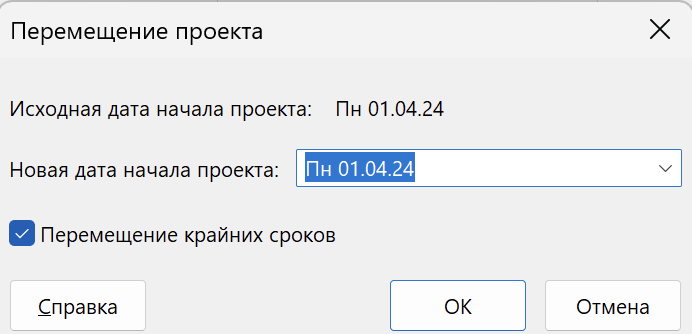
\includegraphics[width=0.75\linewidth]{assets/images/1-start.png}
	\label{fig:r2}
	\caption{Начало проекта}
\end{figure}
\FloatBarrier

Установлена длительность работы в днях, объем работ в часах, а тип задач по умолчанию --- с фиксированными трудозатратами.

\begin{figure}[ht!]
	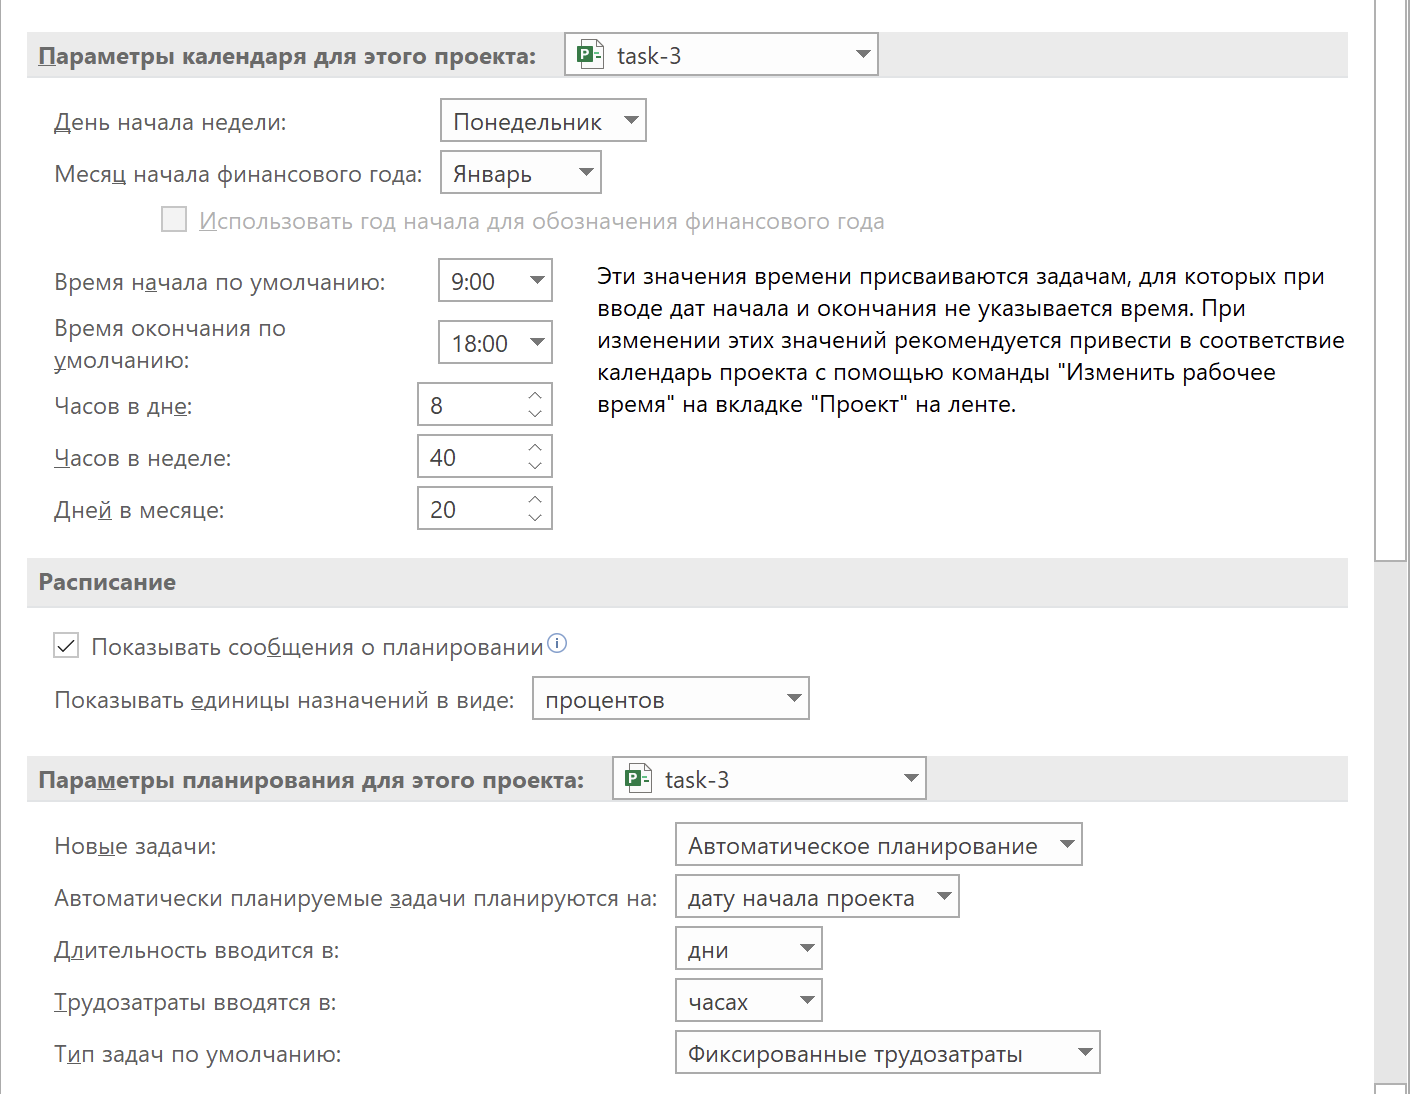
\includegraphics[width=0.75\linewidth]{assets/images/1-long.png}
	\label{fig:r2}
	\caption{Длительность}
\end{figure}
\FloatBarrier

Учтены праздничные дни, попадающие на период реализации проекта.

\begin{figure}[ht!]
	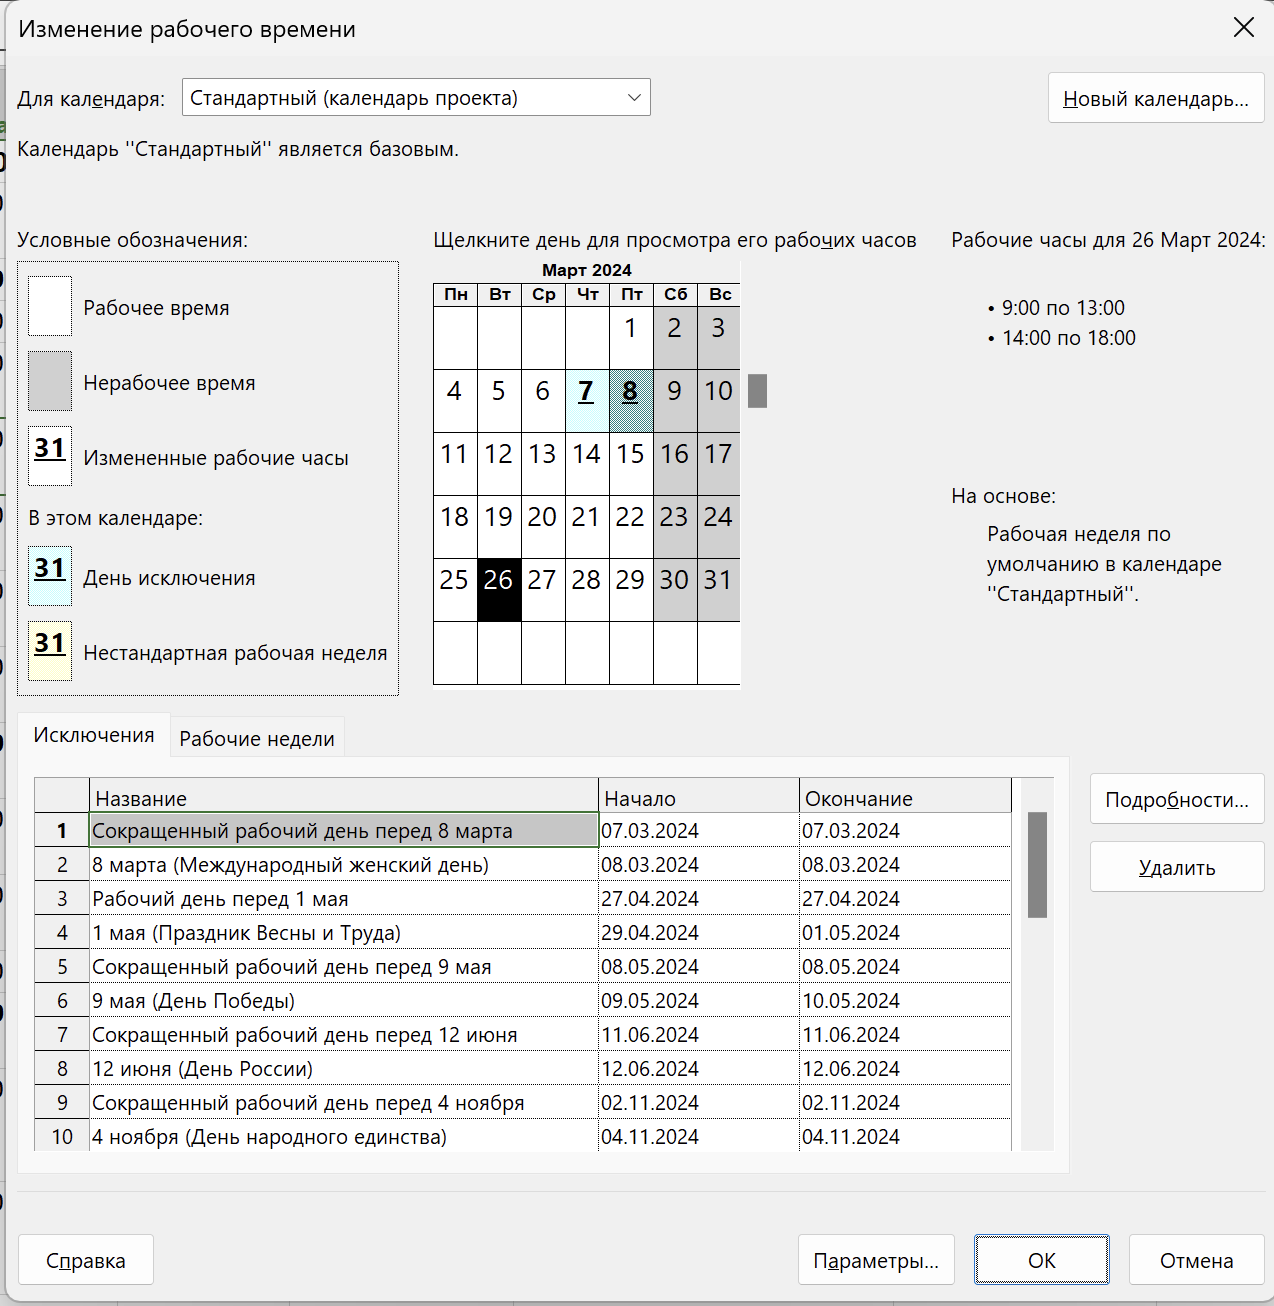
\includegraphics[width=0.75\linewidth]{assets/images/1-calendar.png}
	\label{fig:r2}
	\caption{Календарь}
\end{figure}
\FloatBarrier

\section{Задание 2}

Задачи были заданы в соотвествии с вариантом.

\begin{figure}[ht!]
	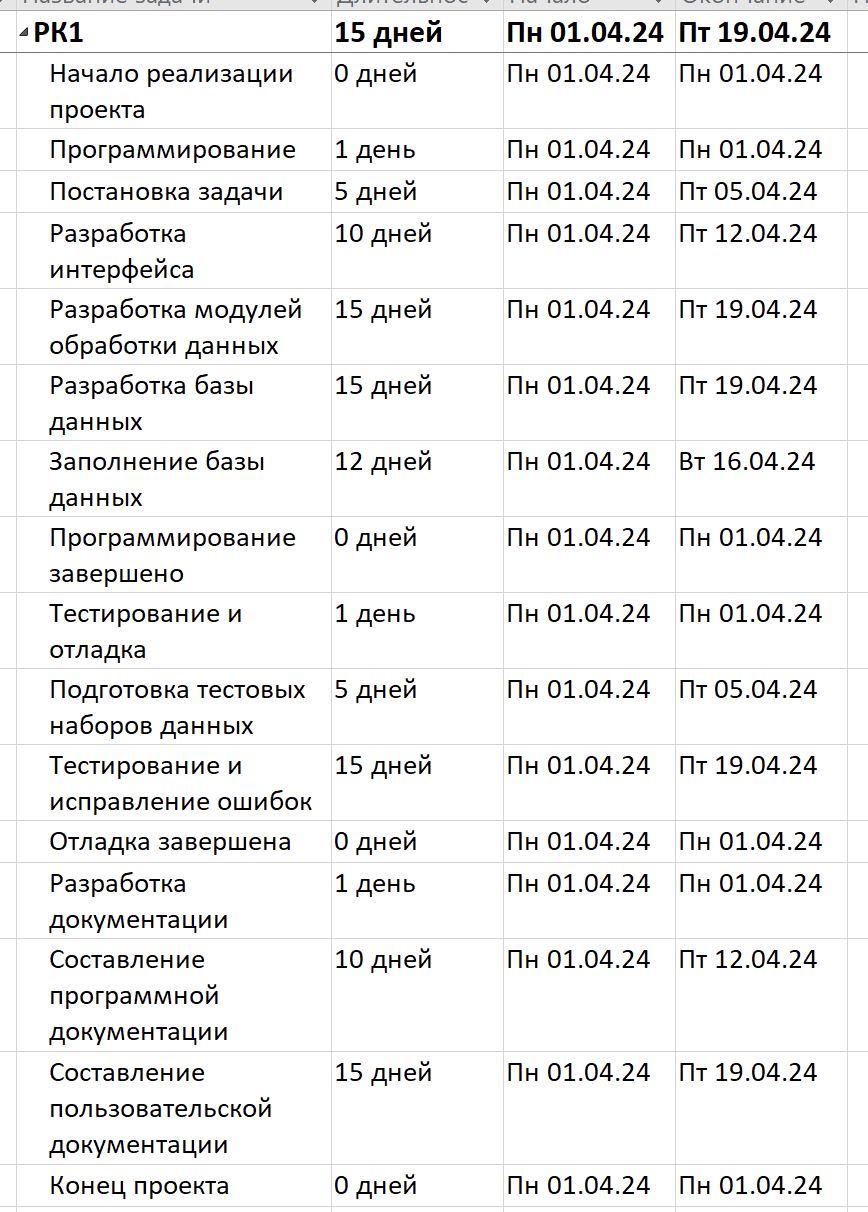
\includegraphics[width=0.75\linewidth]{assets/images/2-tasks.png}
	\label{fig:r2}
	\caption{Задачи}
\end{figure}
\FloatBarrier


\section{Задание 3}

Задачи структурированы.

\begin{figure}[ht!]
	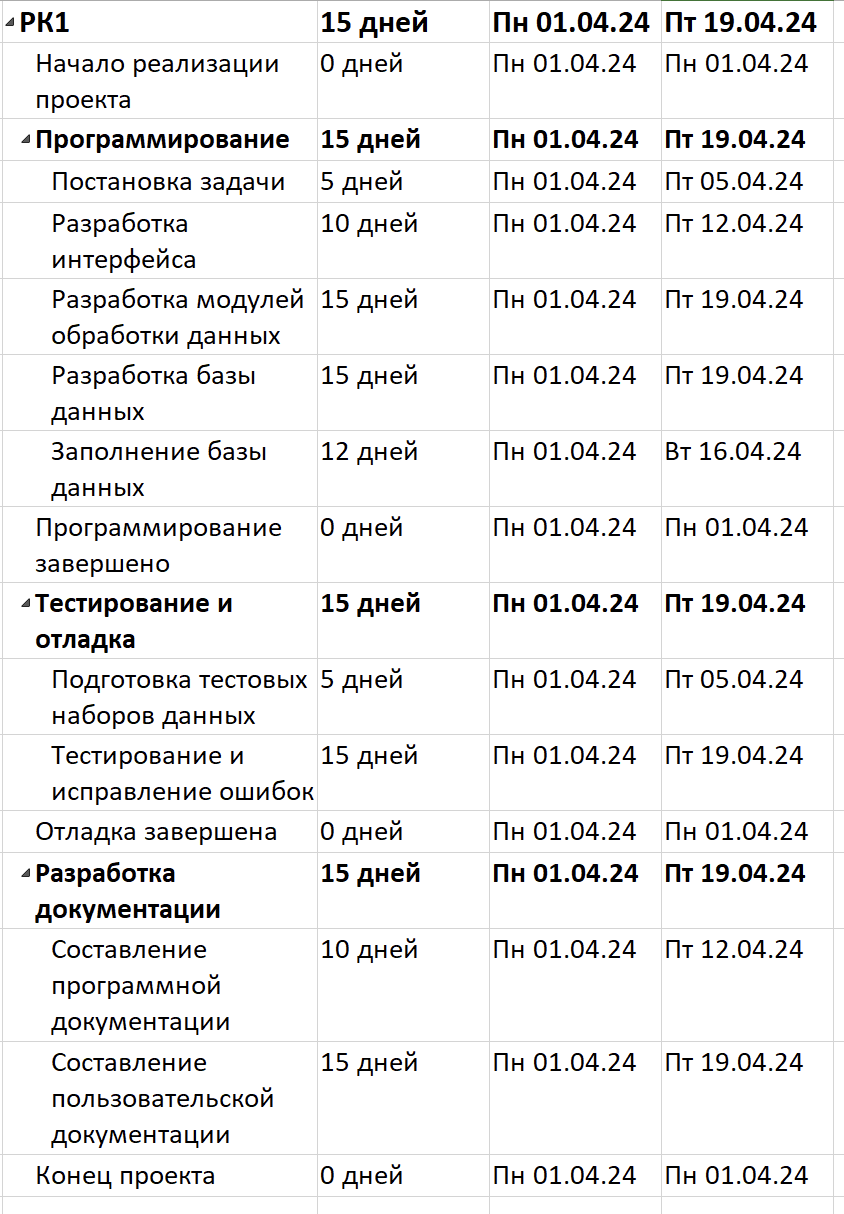
\includegraphics[width=0.75\linewidth]{assets/images/3-tasks.png}
	\label{fig:r2}
	\caption{Задачи}
\end{figure}
\FloatBarrier

\section{Задание 4}

Задачи связаны.

\begin{figure}[ht!]
	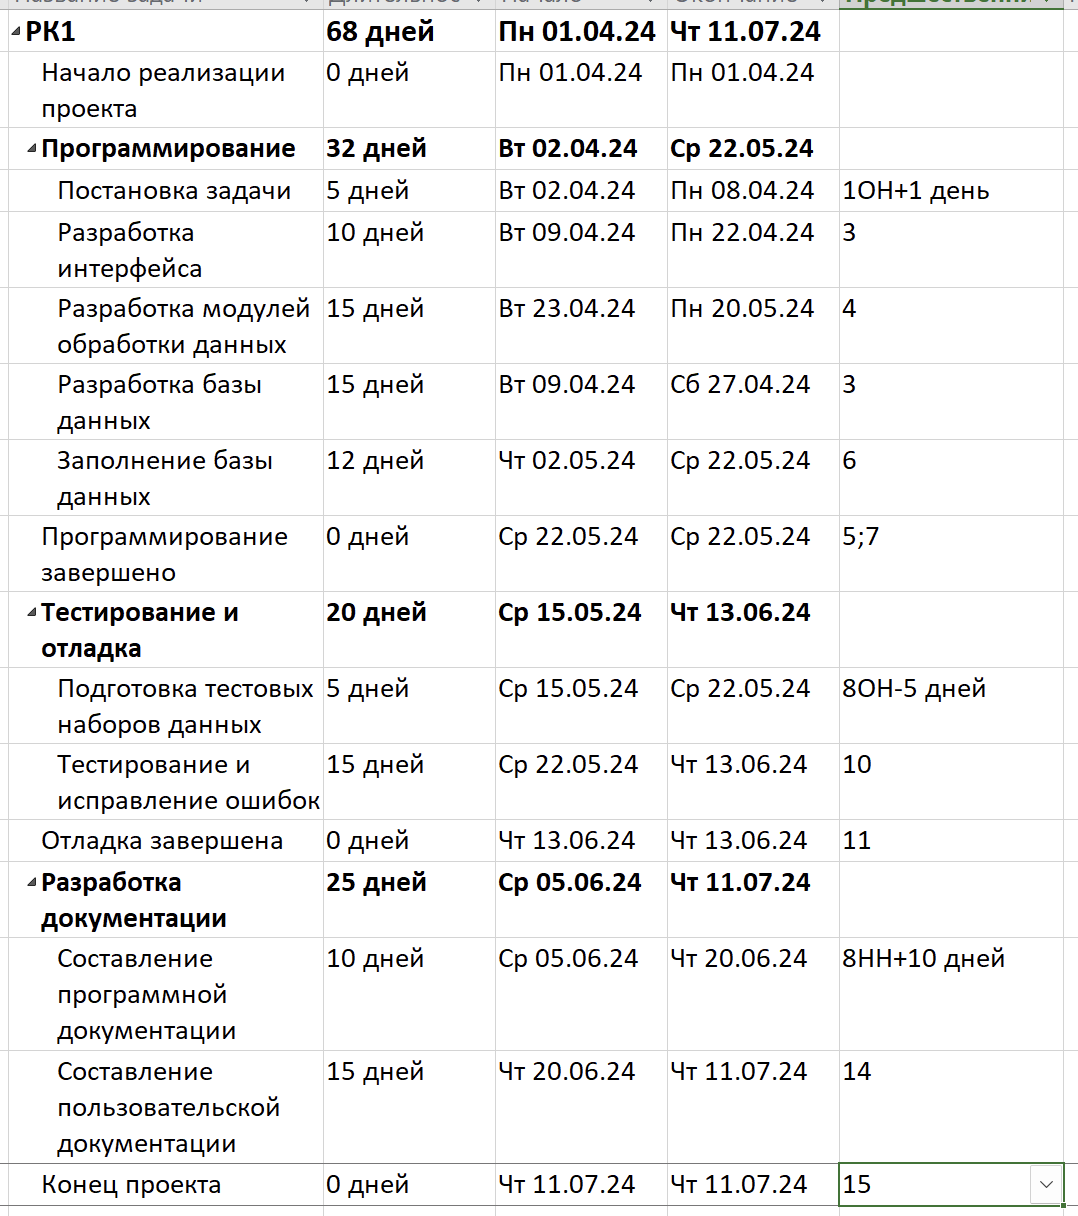
\includegraphics[width=0.75\linewidth]{assets/images/4-task.png}
	\label{fig:r2}
	\caption{Задачи}
\end{figure}
\FloatBarrier


\section{Задание 5}

Назанчены ресурсы в соотвествии с заданием.

\begin{figure}[ht!]
	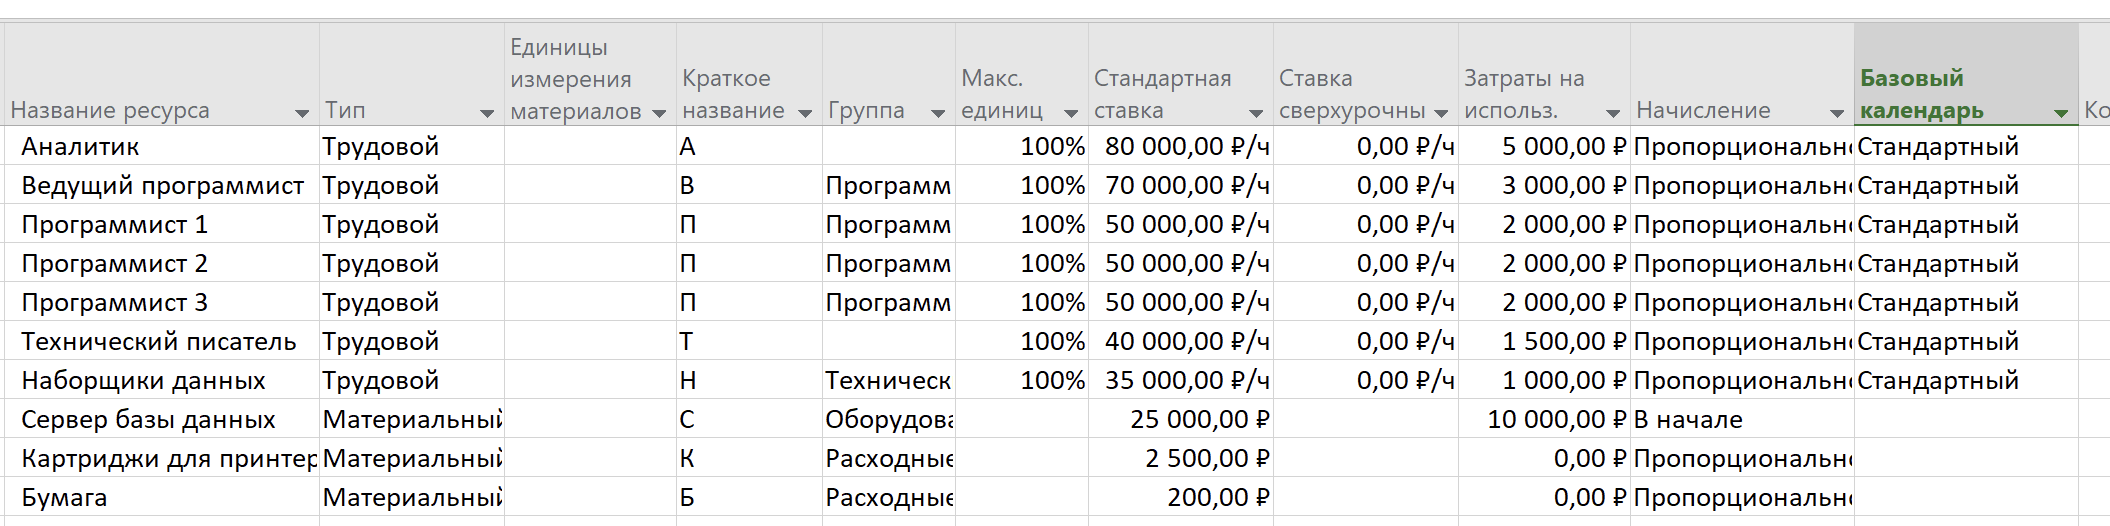
\includegraphics[width=0.75\linewidth]{assets/images/5-task.png}
	\label{fig:r2}
	\caption{Ресурсы}
\end{figure}
\FloatBarrier

\section{Задание 6}

Назаначены ресурсы в сооствествии с заданием, возникли перезгрузки.

\begin{figure}[ht!]
	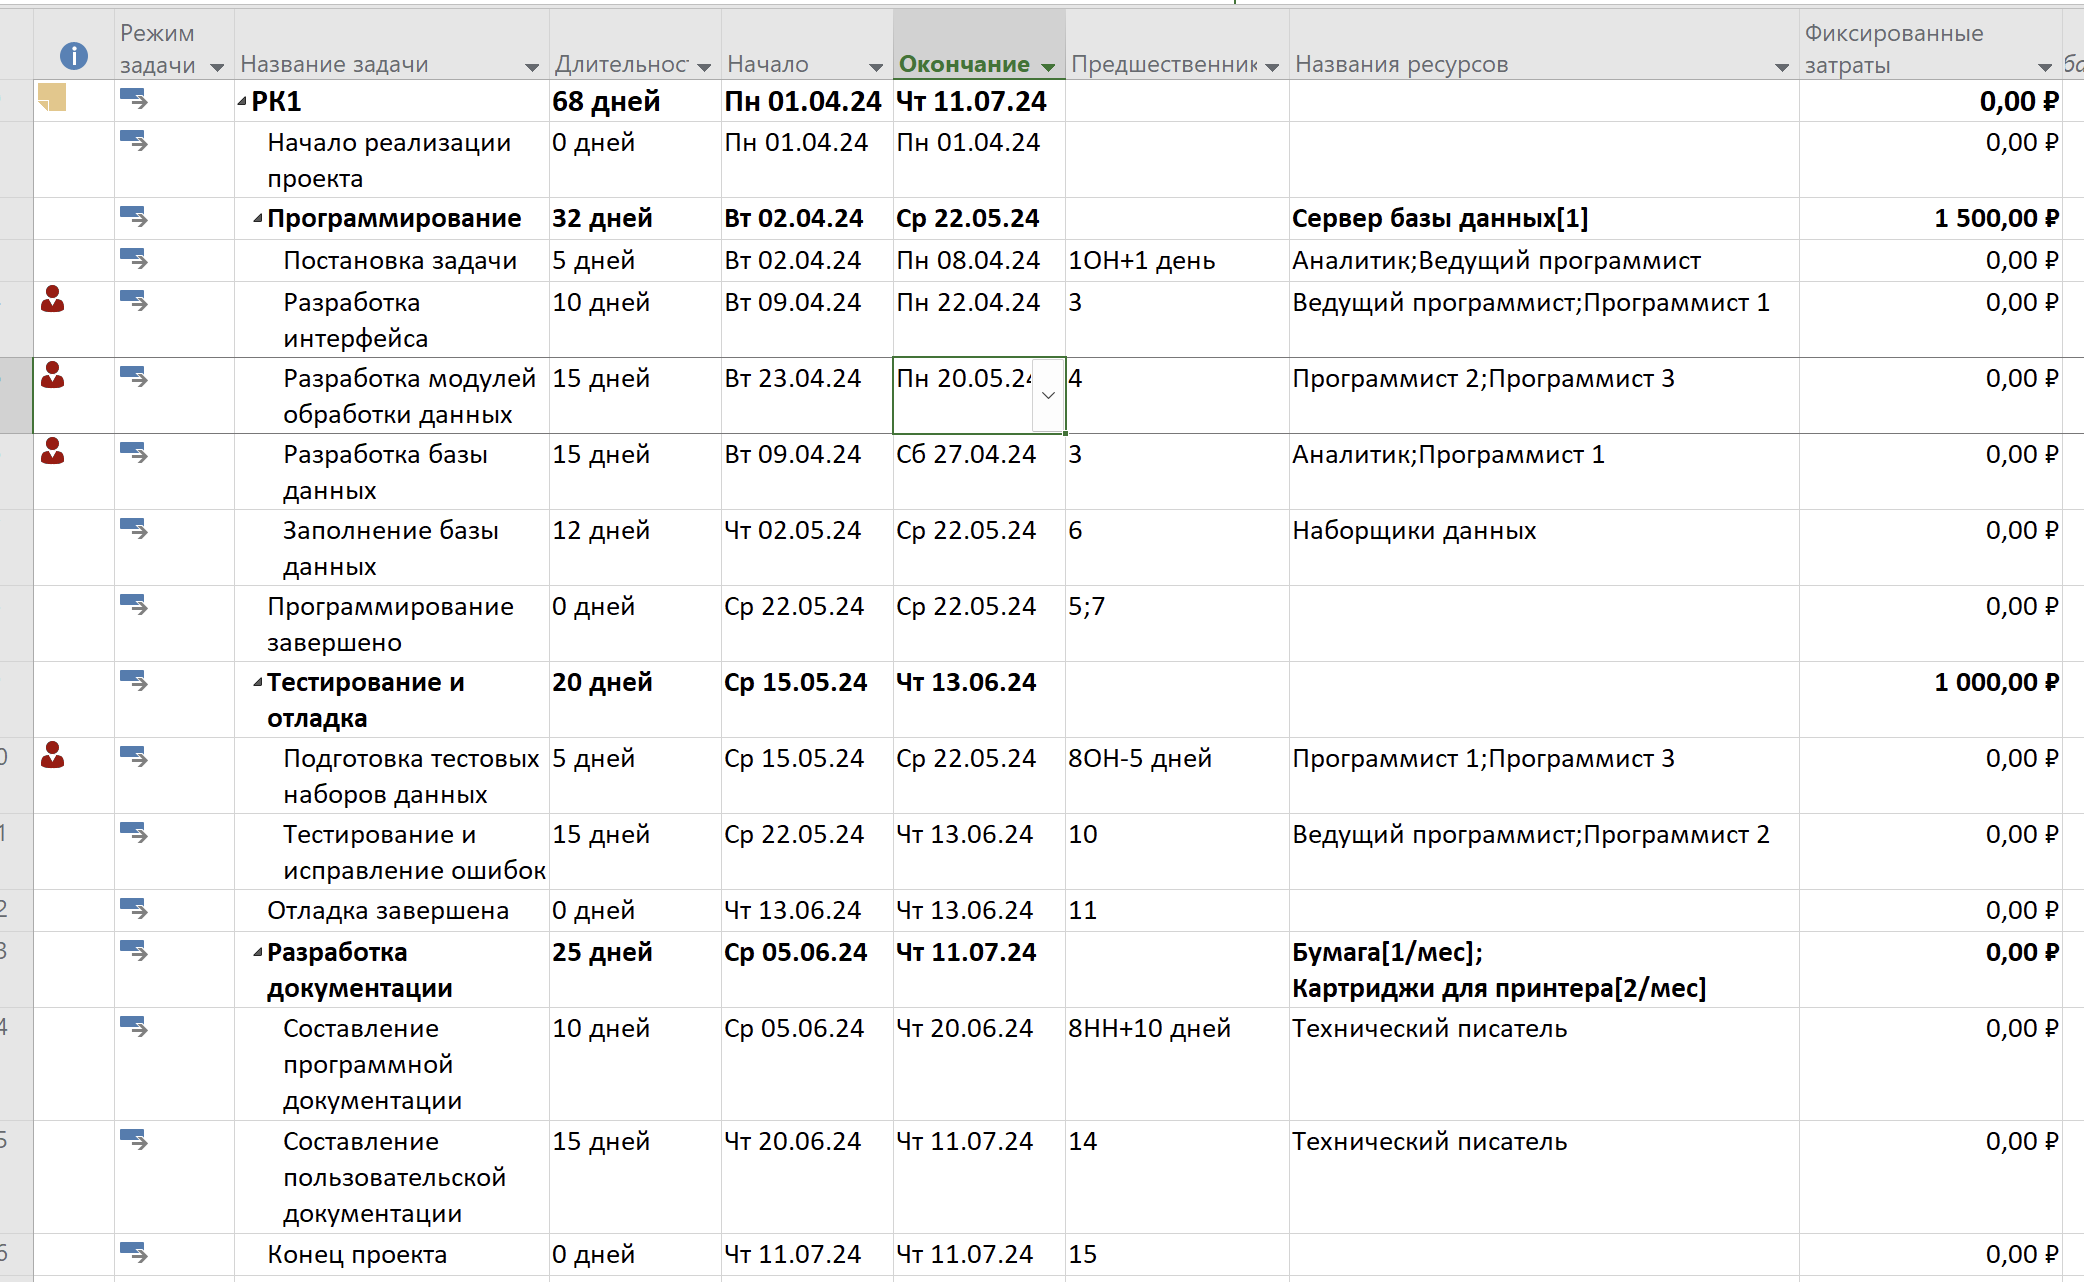
\includegraphics[width=0.75\linewidth]{assets/images/6-tasks.png}
	\label{fig:r2}
	\caption{Ресурсы}
\end{figure}
\FloatBarrier